\chapter{Pulse shape simulation}
\label{cha:pss}
It is proved in the previous chapters that segmented germanium detectors are powerful of distinguishing between single-site events and multi-site events. However, as shown in Fig.~\ref{fig:ph:eve}, (1) there are some multi-site events which are confined to one segment and (2) there are some single-site events that happen on the boundary between two segments. The \textit{boundary events} are rejected erroneously if only single-segment events are collected, because the energy deposited is shared between segments. The analysis of the electrical pulses associated with the events (pulse shape analysis) can help with both problem categories.\footnote{Pulse shape analysis can also help with several other aspects: rejection of background from $\alpha$-particle and neutron interactions with detectors, Compton continuum suppression\cite{comcon}, detection of crystal structure~\cite{agata}, etc.} For events in category (1) the time development of the pulse can reveal a multi-site event; while for events in category (2) the relative strength of the two pulses can reveal whether the interaction position is near the boundary or not. In combination with crystal segmentation, pulse shape analysis plays a crucial role to reach an extremely low background count rate.

Data samples which can mimic the behavior of the $0\nu\beta\beta$ decay events need to be collected in order to estimate the efficiency of the pulse shape analysis. Two data samples commonly used are (1) double escape peak (DEP) events and (2) single Compton scattering events\cite{scoms}. However, the double escape peaks are normally not located near the Q-value of $^{76}$Ge $0\nu\beta\beta$ decay. In addition, the events from the peak are not uniformly distributed throughout the detector crystal\cite{major}. The single Compton scattering events are collected with a very low event rate. The low rate is intrinsic to the measurement and makes it difficult and time consuming to collect samples of satisfactory size. Therefore the data have to be complemented by reliable pulse shape simulation.

The physics models of the drift of electrons and holes inside germanium crystals were established by L. Mihailescu \textit{et al.}\cite{miha} and B. Bruyneel \emph{et al.}\cite{bart}, respectively. The implementation of these models to Siegfried-like detectors are described in detail in this chapter. Some mistakes in Ref.~\cite{miha} are corrected.


\section{Procedure}
\label{sec:pss:proc}
The procedure of the pulse shape simulation\cite{agata} can be described as follows:
\begin{enumerate}
\item Simulate the interactions of particles with germanium detectors using Geant4 to get the spacial distribution and the energy deposits of the interactions (hits);
\item Group hits into one if they are too close to each other (1~mm is used in this work). The position of the new hit is the center of energies of the original hits. The energy of the new hit is the sum of the energies of the original hits.
\item Calculate the number of electron-hole pairs, $n$, created by the hit with energy $E_{\text{hit}}$: $n = E_{\text{hit}} / E_{\text{pair}}$, where the pair energy $E_{\text{pair}} = 2.95$~eV;
\item Calculate the electrical field and weighting potential\cite{Gat82, Rad88, He00} in the detector according to the high voltage applied and the spacial distribution of the impurity;
\item Calculate the drift velocities of the charge carriers taking into account the effect of the germanium crystal structure;
\item Calculate the trajectory of the drift from the interaction point to the boundary of the crystal;
\item Calculate the time development of the charges induced in the electrodes (pulses)\footnote{For segmented detectors, the charges induced in the electrodes of the neighboring segments (transient pulses) can also be calculated.} by the drift of the charge carriers\cite{igex}; 
\item Add to the simulated pulses the effects from the electronics such as the noise, bandwidth limit and the shaping of the pulses, etc.
\end{enumerate}
MaGe, the object-oriented simulation package co-developed by the GERGA and Majorana MC groups as described in Sec.~\ref{sec:ph:sim}, does not only cover the first step but also all the rest aspects of the procedure. The calculation of the electric fields and potentials is described in Sec.~\ref{sec:pss:field}. For the calculation of the drift velocities of charge carriers please see Sec.~\ref{sec:pss:drift}.


\section{Electric and weighting fields}
\label{sec:pss:field}
The electric field $\mathbf{E}$ can be calculated by solving Poisson's equation $\nabla \cdot \mathbf{E} = \frac{\rho}{\epsilon}$ as described in Sec.~\ref{sec:det:field}. However, it is easy to calculate numerically the potential field $\varphi$, which is a number in a certain spacial point, instead of the electric field $\mathbf{E}$, which is a vecter with three components. The electric field $\mathbf{E}$ can be yielded afterwards with the relation $\mathbf{E} = - \nabla \varphi$. Since true coaxial detectors are used it is convenient to rewrite the equation in cylindrical coordinates:
\begin{equation}
\frac{1}{r} \frac{\partial \varphi}{\partial r} + \frac{\partial^{2} \varphi}{\partial r^{2}} + \frac{1}{r^{2}} \frac{\partial^{2} \varphi}{\partial \phi^{2}} +
\frac{\partial^{2} \varphi}{\partial z^{2}} = - \frac{1}{\epsilon_{0}
\epsilon_{R}} \rho,
\label{eq:pss:pocyl}
\end{equation}
where $r, \phi, z$ are the cylindrical coordinates, $\varphi$ and $\rho$ are functions of $r, \phi, z$, $\epsilon_{0}$ and $\epsilon_{R}$ are the dielectric constants in vacuum and germanium, respectively.

The electric field distribution inside the germanium crystal is quite sensitive to the impurity density. Figure~\ref{fig:pss:rho} shows the strength of the electric field as a function of the radius of the detector with the bias voltage fixed to the same value, 3~kV. The electric field changes dramatically with a little change of the impurity.

\begin{figure}[htbp]
\centering
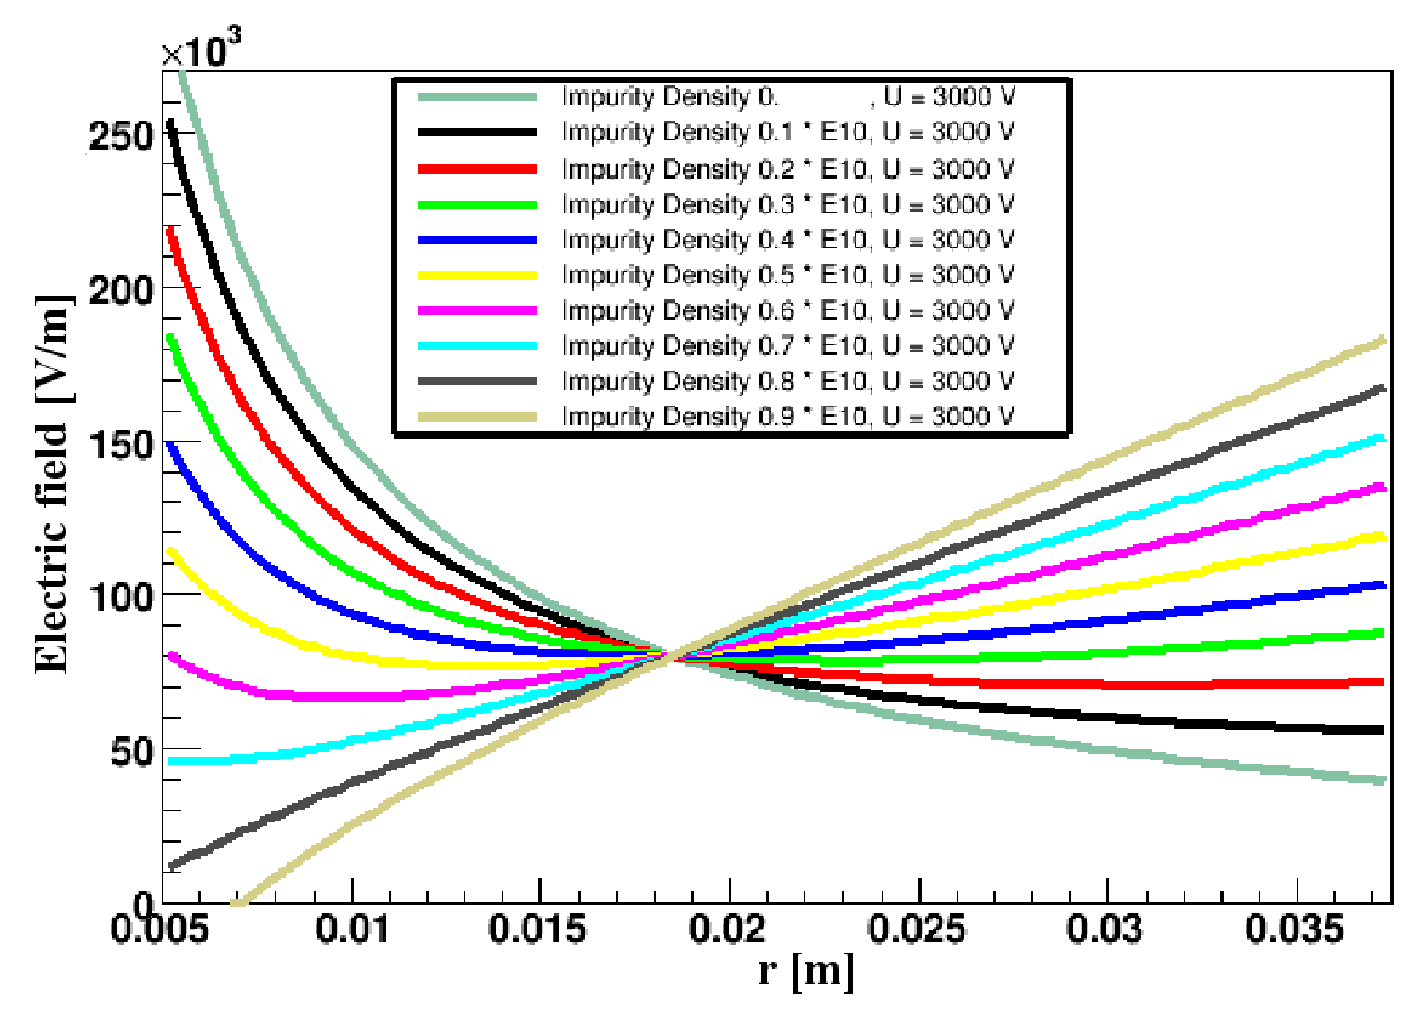
\includegraphics[width=0.7\textwidth]{rho}
\caption{Strength of the electric field as a function of the radius of the detector. It changes dramatically with a little change of the impurity.}
\label{fig:pss:rho}
\end{figure}

The weighting fields and potentials need to be calculated in order to get the induced signals in the electrodes using Shockley-Ramo's Theorem~\cite{Gat82, Rad88, He00} as described in Sec.~\ref{sec:det:ramo}. 

A fine grid inside the detector is defined with certain boundary conditions. The values of potentials in each grid point are updated using the numerical technique \emph{successive overrelaxation}.


\section{Drift of charge carriers}
\label{sec:pss:drift}

\subsection{Mobility}
\label{sec:pss:mobi}
The electron-hole pairs produced by radiations drift to the electrodes of the detector when the bias voltage is applied. The mobility of electrons $\mu_{e}$ and holes $\mu_{h}$ as defined in Sec.~\ref{sec:det:struc} change with the temperature of the germanium crystal. When the temperature of electrons and holes do not differ much from the temperature of the crystal lattice, the drift velocity $\mathbf{v}_{e/h}$ is simply proportional to the electrical field and the crystal structure has no influence. The mobility in this case is just a number $\mu_{e,h} = \mu_{0}$. When germanium detectors are cooled down to, say, liquid nitrogen temperature, the electron-hole pairs are hotter than the crystal lattice. The mobility in this case takes differnt values along different directions and is a complex tersor. The drift tranjectory hence is not always parallel to the electrical field.

Germanium has the same crystalline structure as silicon and diamond, namely, a face-centered cubic (FCC) structure: each atom lies at the center of a regular tetrahedron, and is surrounded at its apices by four atoms, as shown in Fig.~\ref{fig:pss:xtal}.

\begin{SCfigure}[][tbhp]
\centering
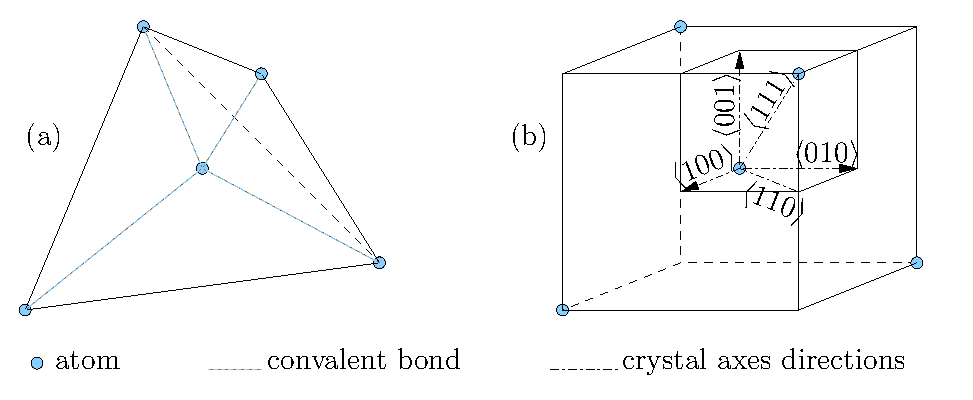
\includegraphics[width=0.6\textwidth]{xtalStruc}  
\caption{Structure of germanium crystal.}
\label{fig:pss:xtal}
\end{SCfigure}

If the electric field lines are parallel with any of the three principal crystallographic axes $\langle 100 \rangle$, $\langle 110 \rangle$ and $\langle 111 \rangle$, the charge carriers will drift along the same direction because of the symmetric structure of the germanium crystal. Though the direction of the drift does not change in this case, the value of the drift velocity does change with the strength of the electric field applied. The relation of the drift velocity with the electric field applied in the axes $\langle 100 \rangle$ and $\langle 111 \rangle$ were measured experimentally. The experiment data can be fitted well with the following parameterization:
\begin{equation}
\label{eq:pss:para}
v = \frac{\mu_{0}E}{[1+(\frac{E}{E_{0}})^{\beta}]^{1/\beta}} - \mu_{n}E,
\end{equation}
where $E, v$ are the magnitudes of the electric field and drift velocity, respectively, $\mu_{0}, \mu_{n}, E_{0}$ and $\beta$ are the parameters to be determined by fitting. The parameter $\mu_{0}$ parametrizes a simple linear relation between $v$ and $E$. The deviation from this linear relation was found at low temperature ($\sim$80~K). It is modeled through the parameters $E_{0}$ and $\beta$. For electric field stronger than 300~V/mm Mihailescu \textit{et al.}~\cite{miha} added the term $\mu_{n}E$ to account for the \emph{Gunn effect} observed by Ottaviani \textit{et al.}~\cite{otta}. This effect is irrelevant to our detectors operated with field strengths between 10~V/mm and 300~V/mm. The values of the parameters fitted with the experimental data are summarized in Table~\ref{tab:pss:pars}. 

\begin{table}[tbhp]
\centering
\caption{Parameters for the experimental drift velocities in the $\langle111\rangle$ and $\langle100\rangle$ directions.}
\label{tab:pss:pars}
\begin{tabular*}{\textwidth}{ccccccc}\hline\hline
Reference & Carrier & Direction & $\mu_{0} \left[ \frac{\mbox{cm}^{2}}{\mbox{V}\cdot\mbox{s}} \right]$ & $E_{0} \left[ \frac{\mbox{V}}{\mbox{cm}} \right]$ & $\beta$ & $\mu_{n} \left[ \frac{\mbox{cm}^{2}}{\mbox{V}\cdot\mbox{s}} \right]$ \\\hline
& Electron & $\langle111\rangle$ & 40180 & 493 & 0.72 & 589 \\
Ref.~\cite{miha}& & $\langle100\rangle$ & 42420 & 251 & 0.87 & 62\\
& Hole & $\langle111\rangle$ & 107270 & 100 & 0.58 & 0 \\
& & $\langle100\rangle$ & 66333 & 181 & 0.744 & 0 \\\hline
& Electron & $\langle111\rangle$ & 38536 & 538 & 0.641 & 510 \\
Ref.~\cite{bart}& & $\langle100\rangle$ & 38609 & 511 & 0.805 & -171\\ 
& Hole & $\langle111\rangle$ & 61215 & 182 & 0.662 & 0 \\
& & $\langle100\rangle$ & 61824 & 185 & 0.942 & 0 \\\hline\hline
\end{tabular*}
\end{table}

Figure~\ref{fig:pss:vvse} visualizes Eq.~\ref{eq:pss:para} with electric field in the range of [7,500]~V/mm. The upper two plots are created using the input parameters provided in Ref.~\cite{miha}, the lower two using the input parameters provided in Ref.~\cite{bart}. The highest curve in each plot (blue in color) is the velocity along the axes $\langle 100 \rangle$. The lowest curve in each plot (red in color) is the velocity along the axes $\langle 111 \rangle$. The drift velocity in any other direction is related to the ones along  $\langle 100 \rangle$ and $\langle 111 \rangle$ axes, hence can be calculated accordingly. The detailed calculation is described in the following sections.

\begin{figure}[tbhp]
\centering
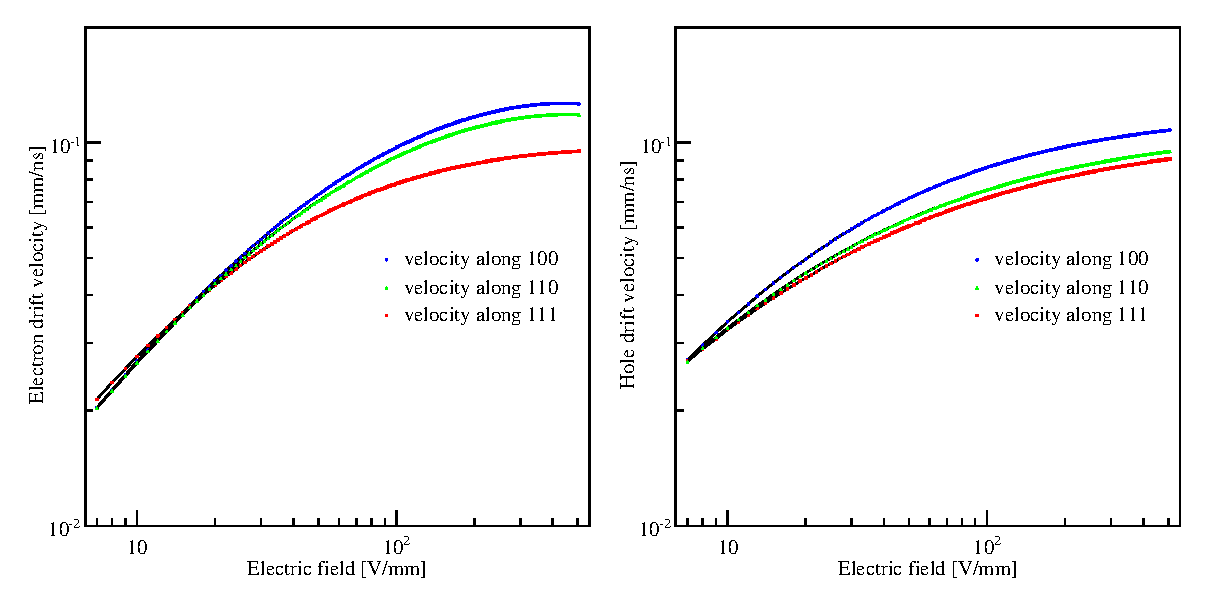
\includegraphics[width=\textwidth]{VvsElucian} \\\hfil
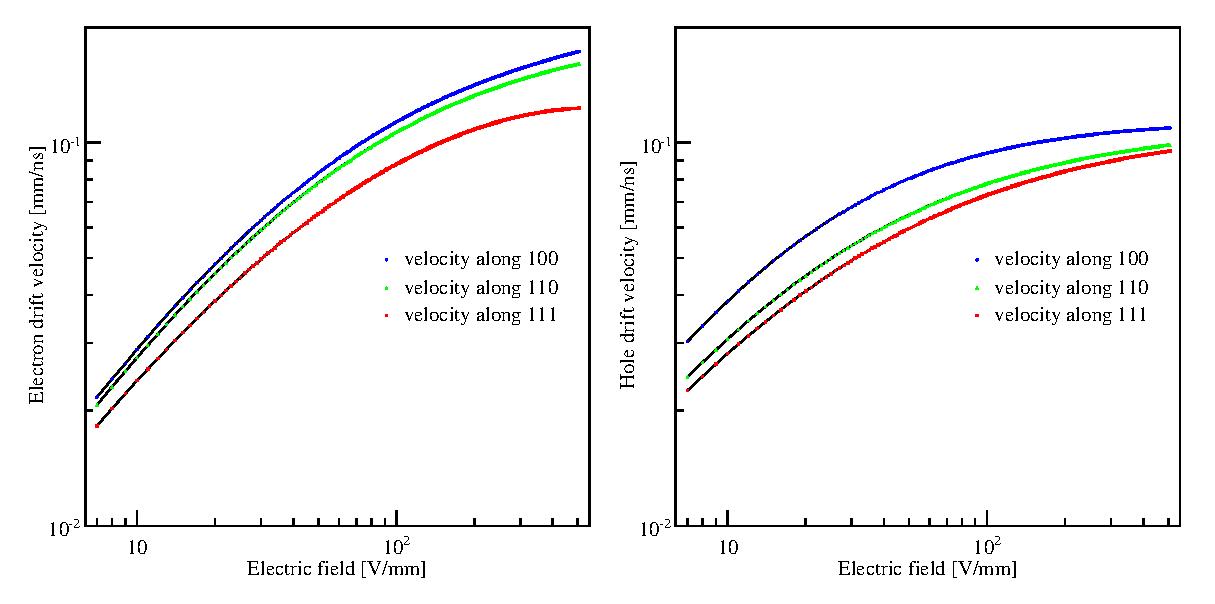
\includegraphics[width=\textwidth]{VvsEbart}
\caption{Drift velocities along the principal crystal axes as functions of electric field in the range of [7,500]~V/mm. Velocities along the axes $\langle 100 \rangle$ and $\langle 111 \rangle$ are calculated with Eq.~\ref{eq:pss:para}, while velocities along $\langle 110 \rangle$ are the simulated results (see Sec.~\ref{sec:pss:elec} and \ref{sec:pss:hole}). The upper plots are created using the input parameters provided in Ref.\cite{miha}, the lower using the input parameters provided in Ref.\cite{bart}.}
\label{fig:pss:vvse}
\end{figure}

\subsection{Coordinate systems}
\label{sec:pss:xyz}
It is very important to distinguish two different coordinate systems in the calculation. One is the coordinate defined by the crystal axes $\langle100\rangle$, $\langle010\rangle$ and $\langle001\rangle$. They are perpendicular to each other hence can be used as the axes of a Cartesian coordinate. The other one, indicated as $xyz$ in Fig~\ref{fig:pss:coo}, is used in Geant4 geometry modeling. Most of the cylindrical coaxial germanium detectors are produced such that their geometric middle axis $z$ is aligned with the crystal axis $\langle 001 \rangle$. The relation between the two coordinate system hence can be simply described by an angle between the $\langle110\rangle$ axis and the y-axis, $\phi_{110}$.
\begin{SCfigure}[][htpb]
\centering
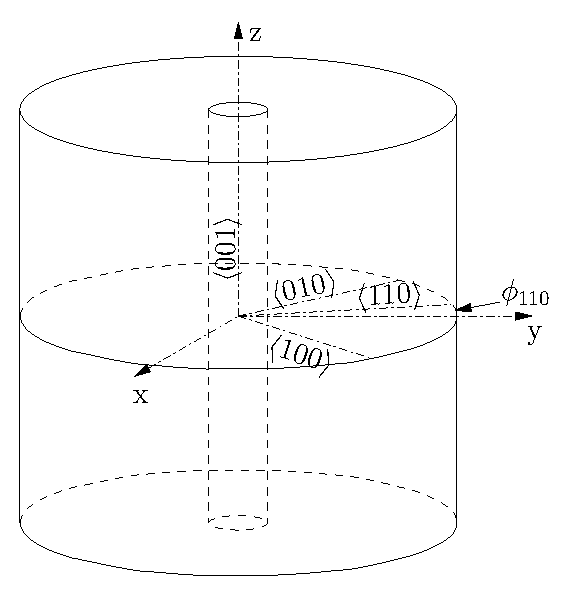
\includegraphics[width=0.4\textwidth]{coordins}  
\caption{The relation between the coordinate $xyz$ used in Geant4 simulation and the one defined by the crystal axes $\langle 100 \rangle$, $\langle 010 \rangle$ and $\langle 001 \rangle$.}
\label{fig:pss:coo}
\end{SCfigure}

\subsection{Electron drift velocity}
\label{sec:pss:elec}
There are four ellipsoidal valleys in the germanium crystal lying along the $\langle111\rangle$ directions as shown in Fig~\ref{fig:pss:valley} taken from Ref.\cite{bart}. 
\begin{SCfigure}[][htpb]
\centering
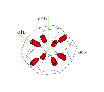
\includegraphics[width=0.4\textwidth]{valleys}  
\caption{Four ellipsoidal valleys along $\langle111\rangle$ directions, where electrons mostly populate (taken from Ref.\cite{bart}).}
\label{fig:pss:valley}
\end{SCfigure}
Electrons mostly populate in them and can be easily accelerated by the electrical field applied. The populations of electrons in other directions are very small, and if they are neglected, the dependence of the electron drift velocity $\mathbf{v}_{e}$ on the applied electric field $\mathbf{E}$ can be written as
\begin{equation}
\label{eq:pss:ed}
\mathbf{v}_{e}(\mathbf{E}) = \mathcal{A}(E) \sum_{j} \frac{n_{j}}{n} \frac{\gamma_{j}\mathbf{E_{0}}}{\sqrt{\mathbf{E_{0}}\gamma_{j}\mathbf{E_{0}}}}, \mbox{ with } j=1,2,3,4,
\end{equation}
where $\mathcal{A}$ is a function of the magnitude of the electric field $E=|\mathbf{E}|$ and temperature, the value of $\mathcal{A}$ must be negative because electrons drift to the opposite direction of the electric field; $\mathbf{E_{0}}$ is the normalized electric field vector; $n_{j}/n$ is the fraction of the carriers (in this case, electrons) in the $j$-th $\langle111\rangle$ valley, $\gamma_{j}$ is the effective mass tensor for the $j$-th $\langle111\rangle$ valley. In the local coordinate of one of the ellipsoidal valleys $x^{\prime}y^{\prime}z^{\prime}$, as shown in Fig.~\ref{fig:pss:axes}, the effective mass tensor has a very simple expression:
\begin{equation}
\label{eq:pss:g0}
\gamma_{0} \equiv \left(
\begin{array}{ccc}
m_{t}^{-1} & 0 & 0 \\
0 & m_{l}^{-1} & 0 \\
0 & 0 & m_{t}^{-1}
\end{array} \right),
\end{equation}
where $m_{t} = 1.64m_{e}$ is the transversal effective electron mass, $m_{l} = 0.0819m_{e}$ is the longitudinal effective electron mass, with $m_{e}$ denoting the free electron mass. Since it is convenient to simulate the interactions and the pulse shape developing in the same coordinate $xyz$, as shown in Fig.~\ref{fig:pss:coo} and \ref{fig:pss:axes}, we have to calculate the expressions of $\gamma_{j}$'s in $xyz$:
\begin{equation}
\label{eq:pss:gs}
\gamma_{j} = R_{j}^{-1}\gamma_{0}R_{j} = R_{j}^{T}\gamma_{0}R_{j},
\end{equation}
where
\begin{equation}
\label{eq:pss:rs}
R_{j} = R_{x^{\prime}}(\arccos(\sqrt{2/3}))R_{z}(\phi_{110}+(j-1)\pi/2)
\end{equation}
is the rotation matrix which could align $\langle111\rangle$ axis to the y-axis. The suffix of $R$'s indicate the rotation axes. The rotation angles are denoted in the brackets following the $R$'s. All the rotations are defined in the counter-clockwise sense.

\begin{SCfigure}[][tbhp]
\centering
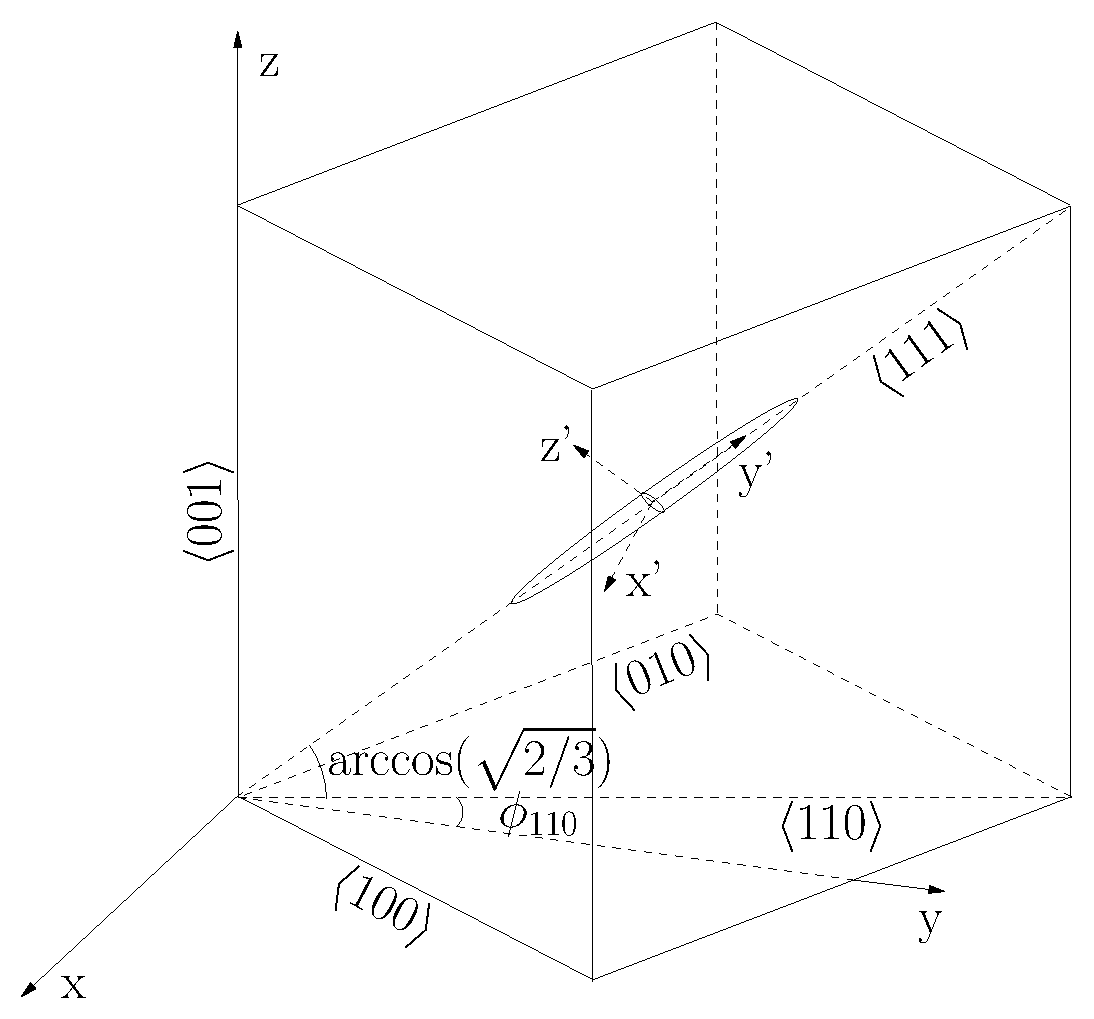
\includegraphics[width=0.4\textwidth]{axes}  
\caption{Relation between the local coordinate $x^{\prime}y^{\prime}z^{\prime}$ of one of the four ellipsoidal valleys and the Geant4 coordinate $xyz$. The $x^{\prime}$ axis is perpendicular to the plane defined by $\langle111\rangle$ and $\langle001\rangle$.}
\label{fig:pss:axes}
\end{SCfigure}

For an experimental determination of the repopulation amplitude, the deviation from a uniform population distribution $n_{e}/n$ (1/4 for germanium) is assumed to vary with the electric field weighted by the factor $\mathcal{R}$:
\begin{equation}
\label{eq:pss:nion}
\frac{n_{j}}{n} = \mathcal{R}(E)   \left[         \frac{\sqrt{\mathbf{E_{0}}\gamma_{j}\mathbf{E_{0}}}}
{\sum_{i}\sqrt{\mathbf{E_{0}}\gamma_{i}\mathbf{E_{0}}}} -               \frac{n_{e}}{n} \right] + \frac{n_{e}}{n}, 
\end{equation}

If the electric field vector is equally oriented with respect to all the $\langle 111 \rangle$ directions, there is an uniform repopulation of the conduction bands, \textit{i.e.} $n_{j}/n = 1/4$. An electric field applied along the $\langle100\rangle$ direction, \textit{i.e.} $\mathbf{E_{0}} = (\sqrt{1/2}, \sqrt{1/2}, 0)^{T}$ in coordinate $xyz$, satisfies this condition. By employing the experimental drift velocity $v_{e}^{100}(E)$ which can be calculated using Eq.~\ref{eq:pss:para}, the absolute value of $\mathcal{A}(E)$ can be calculated as
\begin{equation}
\label{eq:pss:ae}
|\mathcal{A}(E)| = \frac{v_{e}^{100}(E)}  {\displaystyle \sum_{j}     \frac{1}{4} \frac{\gamma_{j}\mathbf{E_{0}}}         {\sqrt{\mathbf{E_{0}}\gamma_{j}\mathbf{E_{0}}}} }, \mbox{ with }       \mathbf{E_{0}} = \left( \begin{array}{c} 
\sqrt{1/2}\\\sqrt{1/2}\\0 \end{array} \right).
\end{equation}

If the electric field vector is oriented along with one of the $\langle 111 \rangle$ directions, \textit{i.e.} $\mathbf{E_{0}} = (0, \sqrt{2/3}, \sqrt{1/3})^{T}$ in coordinate $xyz$, there is an uniform repopulation of the conduction bands among the other three $\langle 111 \rangle$ axes, \textit{i.e.}
\begin{equation}
\label{eq:pss:n111}
\frac{n_{2}}{n} = \frac{n_{3}}{n} = \frac{n_{4}}{n}.
\end{equation}
Since
\begin{equation}
\label{eq:pss:nsum}
\displaystyle \sum_{j}\frac{n_{j}}{n} = 1,
\end{equation}
we have
\begin{equation}
\label{eq:pss:n12}
\frac{n_{1}}{n} + 3\frac{n_{2}}{n}= 1.
\end{equation}
By employing the experimental drift velocity $v_{e}^{111}(E)$ for an applied electric field $E$ in the $\langle 111 \rangle$ direction at a specific temperature, which can be calculated using Eq.~\ref{eq:pss:para}, we have another relation between $n_{1}/n$ and $n_{2}/n$:
\begin{equation}
\label{eq:pss:n12p}
v_{e}^{111}(E) =  \mathcal{A}(E) \left(  \frac{n_{1}}{n} \frac{\gamma_{1}\mathbf{E_{0}}}         {\sqrt{\mathbf{E_{0}}\gamma_{1}\mathbf{E_{0}}}} +  3\frac{n_{2}}{n} \frac{\gamma_{2}\mathbf{E_{0}}}         {\sqrt{\mathbf{E_{0}}\gamma_{2}\mathbf{E_{0}}}} \right).
\end{equation}
One can get the value of $n_{1}/n$ and $n_{2}/n$ by solving the equations \ref{eq:pss:n12} and \ref{eq:pss:n12p} together. Then $\mathcal{R}(E)$ can be calculated as
\begin{equation}
\label{eq:pss:re}
\mathcal{R}(E) = \left( \frac{n_{1}}{n} - \frac{n_{e}}{n} \right) / \left( \frac{\sqrt{\mathbf{E_{0}}\gamma_{1}\mathbf{E_{0}}}}
{\sum_{j}\sqrt{\mathbf{E_{0}}\gamma_{j}\mathbf{E_{0}}}} -       \frac{n_{e}}{n} \right), \mbox{ with } \mathbf{E_{0}} = \left( \begin{array}{c} 
0\\ \sqrt{2/3}\\\sqrt{1/3} \end{array} \right).
\end{equation}

After determination of the parameters $\mathcal{A}$ and $\mathcal{R}$, the drift velocity can be calculated for any direction and any strength of the electric field. The middle curves (green in color) in the left two plots of Fig.~\ref{fig:pss:vvse} are the calculated electron drift velocities along the axis $\langle 110 \rangle$.

\subsection{Hole drift velocity}
\label{sec:pss:hole}
The model used in calculating the hole drift velocity is taken from Ref.~\cite{bart}. In this model only the \emph{heavy hole valence band} is responsible for the anisotropic mobility while the other effects are neglected. The holes are accelerated in the electrical field until their energies become 0.037~eV. At this point they are very likely to emit optical phonons. By doing so the holes lose most of their energies and resume acceleration in the field direction and a new cycle starts. 

The probability of finding a heavy hole in a specific momentum state $\mathbf{k}$ reaches its maximum in the direction parallel to the electric field. The mean wave vector $\mathbf{k}_{0}(k_{0}, \theta_{0}, \phi_{0})$ is then assumed to be aligned with the electric field $\mathbf{E}(E, \theta, \phi)$, \textit{i.e.} $\theta_{0} = \theta, \phi_{0} = \phi$, where $\theta, \phi$ are the polar and azimuthal angles with respect to the coordinate defined by the $\langle 100 \rangle$, $\langle 010 \rangle$ and $\langle 001 \rangle$ axes as shown in Fig.~\ref{fig:pss:vsphere}.

\begin{SCfigure}[][tbhp]
\centering
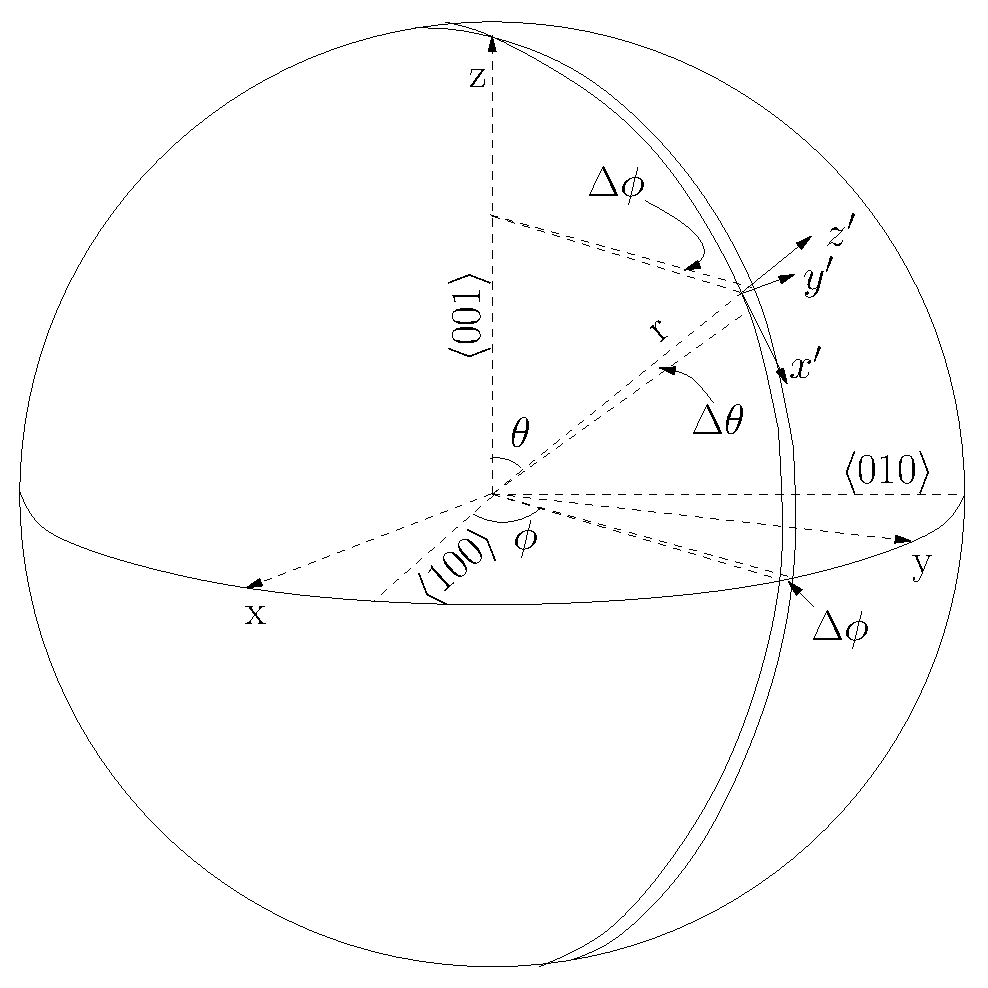
\includegraphics[width=0.4\textwidth]{vsphere}  
\caption{Relation between the coordinate defined by the crystal axes $\langle100\rangle$, $\langle010\rangle$ and $\langle001\rangle$, the one used in the Geant4 simulation $xyz$ and the local coordinate $x^{\prime}y^{\prime}z^{\prime}$ attached to each position.}
\label{fig:pss:vsphere}
\end{SCfigure}

The three components $(v_{x^{\prime}}, v_{y^{\prime}}, v_{z^{\prime}})^{T}$ of the hole drift velocity $\mathbf{v}$ in the local coordinate $x^{\prime}y^{\prime}z^{\prime}$ at any position $(r, \theta, \phi)$ (as shown in Fig.~\ref{fig:pss:vsphere}) can be expressed as:
\begin{equation}
\label{eq:pss:vsphere}
\begin{array}{rcl}
v_{x^{\prime}} = v_{r} &=& v^{100}_{h}(E)[1-\Lambda(k_{0})(\sin(\theta)^{4}\sin(2\phi)^{2} + \sin(2\theta)^{2})],\\
v_{y^{\prime}} = v_{\theta} &=& v^{100}_{h}(E)\Omega(k_{0})[2\sin(\theta)^{3}\cos(\theta)\sin(2\phi)^{2} + \sin(4\theta)],\\
v_{z^{\prime}} = v_{\phi} &=& v^{100}_{h}(E)\Omega(k_{0})\sin(\theta)^{3}\sin(4\phi).
\end{array}
\end{equation}
The mean wave number $k_{0}$ can be expressed as a function of $v_{rel} = v^{111}_{h}(E)/v^{100}_{h}(E)$:
\begin{equation}
\label{eq:pss:k0}
k_{0}(v_{rel}) = 9.2652 - 26.3467v_{rel} + 29.6137v_{rel}^{2} - 12.3689v_{rel}^{3},
\end{equation}
where $v^{111}_{h}(E)$ and $v^{100}_{h}(E)$ are the drift velocities along the $\langle111\rangle$ and $\langle100\rangle$ axes. They can be calculated using Eq.~\ref{eq:pss:para}. The function $\Lambda$ and $\Omega$ govern the amplitude of the anisotropy and can be expressed as
\begin{equation}
\label{eq:pss:lamb}
\Lambda(k_{0}) = -0.01322k_{0} + 0.41145k_{0}^{2} - 0.23657k_{0}^{3} + 0.04077k_{0}^{4},
\end{equation}
\begin{equation}
\label{eq:pss:ome}
\Omega(k_{0}) = 0.006550k_{0} - 0.19946k_{0}^{2} + 0.09859k_{0}^{3} - 0.01559k_{0}^{4}.
\end{equation}

The three components $(v_{x}, v_{y}, v_{z})^{T}$ of the hole drift velocity $\mathbf{v}$ in the coordinate $xyz$ (as shown in Fig.~\ref{fig:pss:vsphere}) can be calculated as:
\begin{equation}
\label{eq:pss:v2v}  
\left(
\begin{array}{c}
v_{x} \\ v_{y} \\ v_{z}
\end{array}
\right) = R_{z}(\phi + \frac{\pi}{4} + \phi_{110}) R_{y^{\prime}}(\theta) \left( 
\begin{array}{c}
v_{x^{\prime}} \\ v_{y^{\prime}} \\ v_{z^{\prime}}
\end{array} \right),
\end{equation}
where $R$'s indicate the rotation matrix along a specific axis, such as $y^{\prime}$ or $z$. The rotation angles are denoted in their following brackets. All the rotations are defined in the counter-clockwise sense. The middle curves (green in color) in the right two plots of Fig.~\ref{fig:pss:vvse} are the calculated hole drift velocities along the axis $\langle 110 \rangle$.


\section{Trajectory of drift}
\label{sec:pss:trj}
The displacement vector $\Delta \mathbf{r}$ that a charge carrier drifts within a short time interval $\Delta t$ can be calculated once the drift velocity vector $\mathbf{v}_{i}$ in the original position $\mathbf{r}_{i}$ is deduced using the method described in the previous two sections. The new position $\mathbf{r}_{i+1}$ is then
\begin{equation}
\label{eq:pss:pos}
\mathbf{r}_{i+1} = \mathbf{r}_{i} + \Delta \mathbf{r} \ \ (i=0,1,...), \text{ with } \Delta \mathbf{r} = \mathbf{v}_{i} \Delta t.
\end{equation}
This position updating process continues until the charge carrier reach the boundary of the crystal. The series of position vector $\mathbf{r}_{i}$ from $\mathbf{r}_{0}$ to $\mathbf{r}_{\text{boundary}}$, $(\mathbf{r}_{0}, \mathbf{r}_{1}, ..., \mathbf{r}_{i}, ..., \mathbf{r}_{\text{boundary}})$, depicts the trajectory of the drift of the charge carrier.

Two different numerical methods are used to calculate the trajectory. One is the Eular method, the other is the 4$^{th}$ Ronge-Kutta method. The former is fast in calculation but less precise. However, when the time interval $\Delta t$ goes smaller than 1~ns, the difference between the two methods is tiny.

Figure~\ref{fig:pss:trjs} shows the drift trajectories projected on the x-y cross sections of Siegfried-like detectors. The crystal axis $\langle 110 \rangle$ is assumed to be parallel to the x-axis (\textit{i.e.}, $\phi_{110}$ as shown in Fig.~\ref{fig:pss:coo} is set to be zero). The left plot shows the drift of electrons starting from the outer surface of the detector to the inside. The start points are distributed along the outer circle with equal distance between each other. The right plot shows the drift of holes starting from the inner surface to the outside. The start points are distributed along the inner circle with equal distance between each other. The bias voltage is set to be 3000~V on the core of the detector. The time window set in the calculation is 400~ns. All the electrons reach the inner surface within this time window, but not all the holes reach the outer surface. This is because electrons drift faster than holes, and holes drift slowest along $\langle 110 \rangle$ direction, as also shown in Fig.~\ref{fig:pss:vvse}.
\begin{figure}[tbhp]
\centering
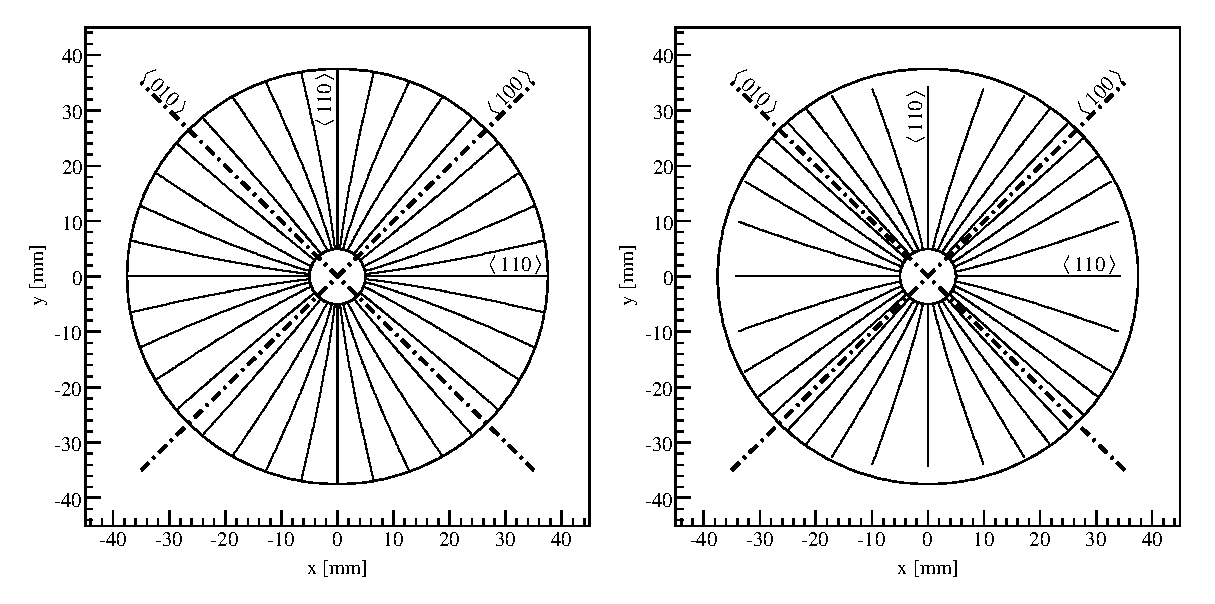
\includegraphics[width=\textwidth]{trjs}
\caption{Drift trajectories projected on the x-y cross sections of Siegfried-like detectors. Detailed explanation please refer to the text.}
\label{fig:pss:trjs}
\end{figure}

The trajectories along the crystal axes are straight as explained in Sec.~\ref{sec:pss:mobi}. However, they are clearly bend along other directions. This causes different occupancies in different segments as shown in Fig.~\ref{fig:ph:mcb}. The crystal axis orientation can be deduced by comparing the occupancy distributions of data and MC. This is described in detail in the next chapter.


\section{Raw pulse shapes}
\label{sec:pss:ps}
Once the weighting fields and potential, the drift velocities and trajectories of the charge carriers are known, Eq.~\ref{eq:det:ramoq} and \ref{eq:det:ramoi} introduced in Sec.~\ref{sec:det:ramo} can be used to calculate the time development of the induced charge $Q(t)$ or current $I(t)$ in each electrode (raw pulses in short). Figure~\ref{fig:pss:pss} shows the raw charge and current pulses induced in segment A, B, C and the core of a Siegfried-like detector by a hit shown in Fig.~\ref{fig:pss:psh}. The colored contour in Fig.~\ref{fig:pss:psh} shows the weighting potential of segment B, the dashed line shows the drift trajectory of holes and the dotted line shows the drift trajectory of electrons. The amplitude of the transient pulse induced in segment A is larger than that in segment C because the trajectory of the hit in segment B is closer to segment A than to segment C.
\begin{figure}[htbp]
\centering
\subfloat[Weighting potential]{\label{fig:pss:psh}
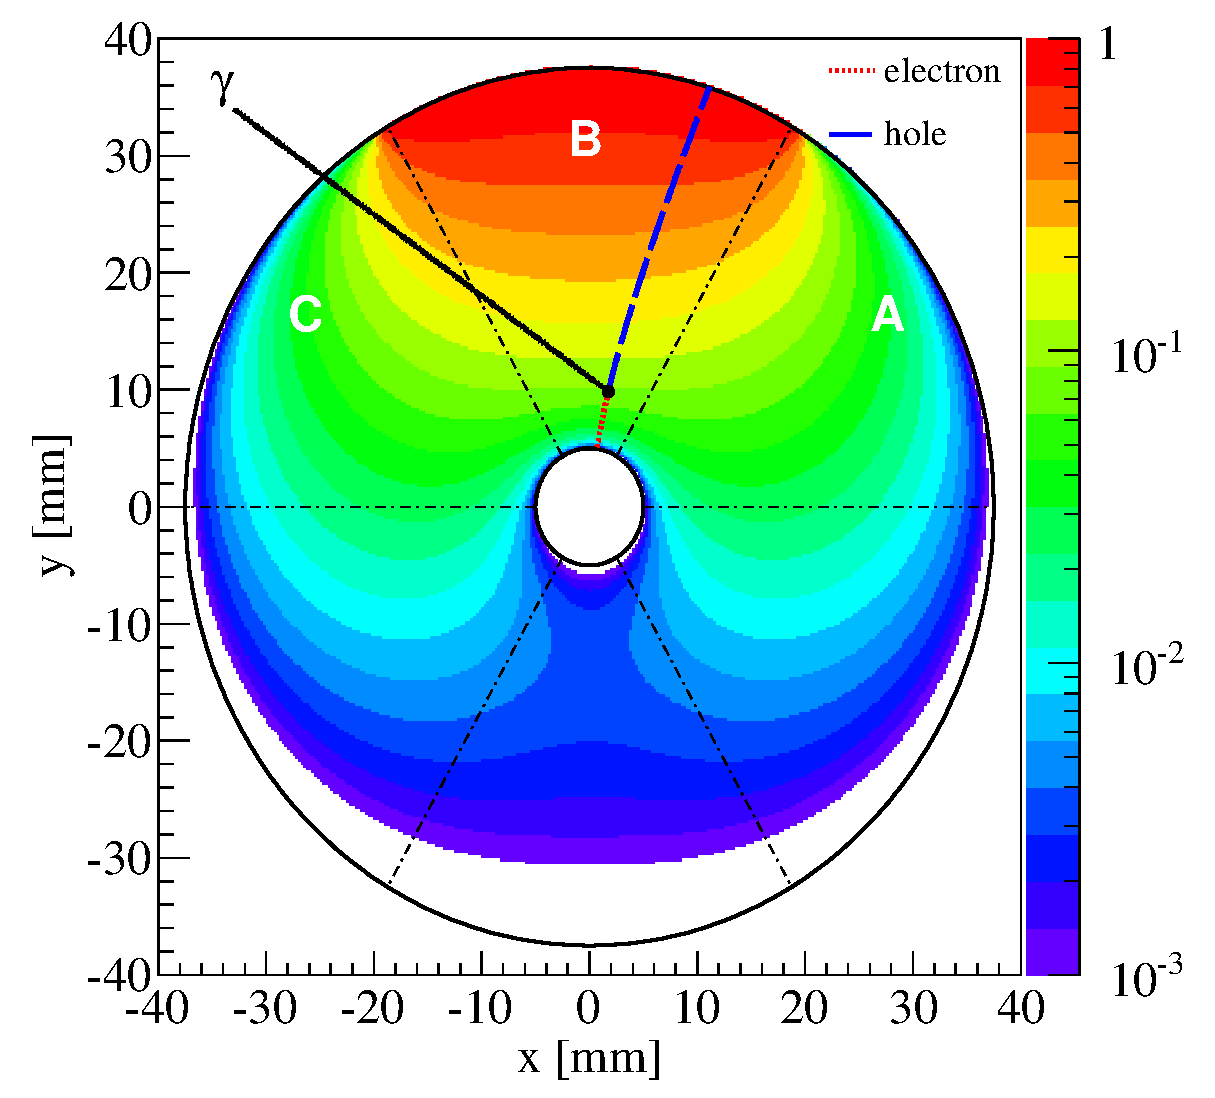
\includegraphics[height=0.22\textheight]{WP}}%
\subfloat[Simulated charge and current pulses]{\label{fig:pss:pss}
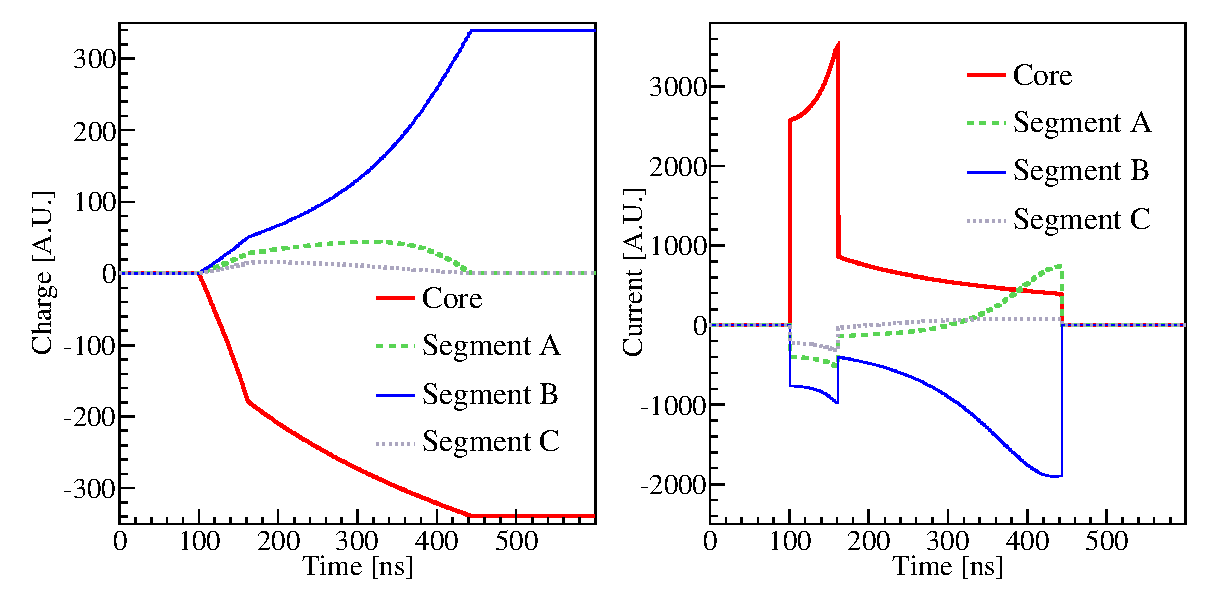
\includegraphics[height=0.22\textheight]{CIPS}}%
\caption{Simulated charge and current pulses induced in segment A, B, C and the core of a Siegfried-like detector.}
\label{fig:pss:ps}
\end{figure}


\section{Effects of electronics}
\label{sec:pss:dbn}
The pulses recorded by the DAQ system are quite different from the raw pulses. Not only their amplitudes but also their shapes are changed by the electronics. For example, the limit on the bandwidth of the signal transmission through the electronics cut off the signal components with frequency higher than the limit. The sharp changes in a pulse are hence smeared. The baseline after a pulse decrease exponentially to its original level with a time constant $\tau$. This also needs to be simulated. The electric noise may destroy any fine structure of a pulse, hence also needs to be simulated.

Figure~\ref{fig:pss:elec} shows the changes of a raw pulse after folded in the effects from the limit of the transmission bandwidth, the decay of the baseline and the noise. The cut-off bandwidth set in the simulation is 10~MHz, the decay time is $5 \mu$s, and the noise level is 5\% of the pulse amplitude. These values are set larger than those in the test stands introduced before in order to show the effect clearly.
\begin{SCfigure}[][htbp]
\centering
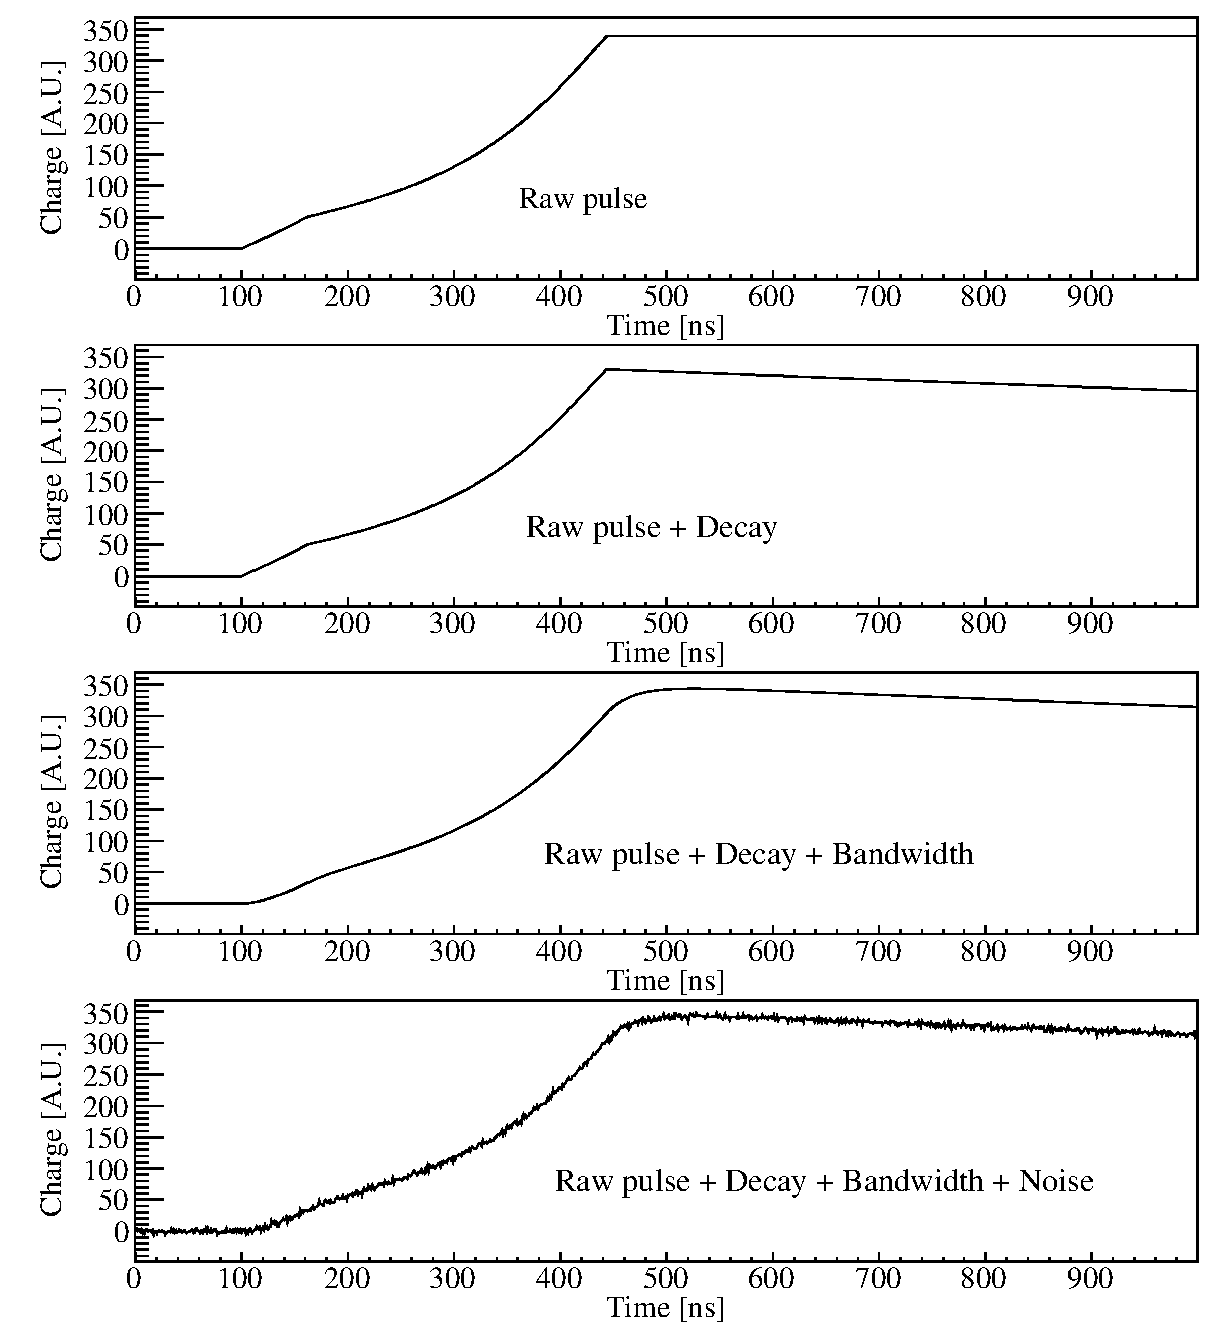
\includegraphics[width=0.5\textwidth]{PSDBN}
\caption{Changes of a raw pulse after folded in the effects from the limit of the transmission bandwidth, the decay of the baseline and the noise.}
\label{fig:pss:elec}
\end{SCfigure}


%%% Local Variables:
%%% mode:latex
%%% TeX-master: "thesis"
%%% End:
